\chapter{UAS-enabled WiSAR Proposal} \label{app:uas_wisar}

This appendix is a proposal to create a UAS for the UE-WiSAR domain.  This represents the initial step towards our ultimate goal of reducing the number of humans in a UAS.  During the requirement gathering and design phase of the project it became clear that in a system this complex the right design was paramount to success.  Instead of blindly pressing forward with the software development we decided that the more important scientific problem was to figure out how to model and validate the system design before implementation.  

\section{INTRODUCTION}
Advances in Micro Unmanned Aerial Vehicle (mUAV) technology has pushed mUAVs
into new frontiers.  UAV Enabled Wilderness Search and
Rescue (UE-WiSAR), one of these frontiers, has been a focus of the Human
Centered Machine Intelligence (HCMI), Multiple Agent Intelligent Coordination and Control (MAGICC) and Computer Vision (CV) labs at Brigham Young University since 2005.  In that time research has
been conducted on human interaction with mUAVs, improving target detection by
enhancing video taken from a mUAV, integrating mUAVs into a SAR environment,
and improving the mUAVs chance of getting video footage of the target.  Over
the course of this research many of the ideas for improving UE-WiSAR results
have been validated through simple experiments and user studies.  Live Field
Demo's with actual Search and Rescue personnel have also shown favourable
results. These results represent important progress in Human Robot Interaction. 

Although the research has proven successful, many of the tools developed for
UE-WiSAR are unfit to share with a broader community.  This proposal outlines
the challenges faced by UE-WiSAR, the solutions discovered for overcoming these
challenges and a plan for creating UE-WiSAR software that incorporates said
solutions into a stable software package as part of an industrial thesis.  As an
industrial thesis the emphasis is not on new research but on delivering high
quality software

\section{PREVIOUS WORK}
One goal of this project is to take past research and present it in a software
application that encourages future researchers to use the software as a
framework for continued research.  Essentially what this means is that the
entire purpose of developing the UE-WiSAR software is to make it available
to future researchers and, more importantly, practicing searchers.  The majority
of the referenced work comes from a combined effort from the HCMI, MAGICC, and CV labs at BYU and focuses on solving
the specific problems that arise when bringing a small UAV into the WiSAR arena.
This proposal represents the realization of this goal
\cite{lin2010supporting}.
  
  
\section{WiSAR}
\subsection{The Problem}
Wilderness Search and Rescue (WiSAR) is more prevalent today then in any other
time in history.  While Search and Rescue has been around since the beginning of
mankind \cite[p.~13]{setnicka1980}, the improved communications and increased
accessibility to wilderness areas have caused an increase need for WiSAR
operations.  Often times these operations have limited resources due to limited
funds, remote locations, and dangerous conditions.

% Furthermore, the paradigm shift that government agencies,
% instead of the individual, are responsible for personal
% safety \cite[p.~viii]{setnicka1980} has created a strain on local government
% agencies to provide effective SAR operations.  To add to this pressure a
% prolonged WiSAR operation can be exorbitantly expensive ``citation''.  This
% increasing pressure has prompted research to provide more effective SAR tools
% while lowering SAR costs.

\subsection{Concepts}
% Search and Rescue implies searching for an individual and then rescuing them
% once found.  With UAV's this is slightly different.  These UAV's will probably
% never be capable of performing the actual rescue.  This means that while
% classified as Search and Rescue the role performed by the UAV is strictly a
% searching role.  This means that UE-WiSAR is not necessarily useful for all
% WiSAR operations.  

To help understand how UE-WiSAR will be effective, some WiSAR
concepts, defined by T.J. Setnicka \cite[p.~35]{setnicka1980}, will be used. 
The first concept is the four core elements of a WiSAR operation.
\begin{figure}[h]
	\begin{center}
		\begin{math}
			Locate \Rightarrow Reach \Rightarrow Stabilize \Rightarrow Evacuate
		\end{math}
	\end{center}
	\caption{Core SAR Elements}
\end{figure}

The second concept is the WiSAR plan and its components, specifically Strategy
and Tactics.  Strategy is the process of gathering information and making an
accurate assessment of the situation.  Tactics are outlined solutions for
specific situations that can be used as part of a Strategy.


% This basic understanding of WiSAR core elements and
% plan components are important to understand the definitions referred to
% throughout this proposal.  These concepts represent how UE-Wisar software will
% be effective in traditional WiSAR operations.

\subsection{Searching}
% In each WiSAR operation the time spent in each of the core elements is
% different.  Some operations may spend the majority of time in reaching and
% evacuating the person.  No other SAR elements can be accomplished, however,
% until the person is located.  This typically represents the majority of time
% spent if the person is missing.  Locating an individual in the wilderness can be
% a daunting task.  SAR commanders develop Strategies for locating the person and
% use the Tactics available to them as part of those Strategies.  Each Tactic
% applied to a search is based on availability, effectiveness, and cost.  One
% Tactic that has proven it's effectiveness is aerial surveillance.  One large
% drawback to this Tactic is the cost.  Until recently most aerial surveillance
% has been done with piloted aircraft.  Advances in Unmanned Aerial Vehicles (UAV)
% have created new options for providing aerial surveillance, however, high-end
% commercial UAV's are still incredibly expensive.  This has prompted a deeper
% look into mUAV which are low-cost but by their very nature have a long list of
% obstacles that need to be overcome before they can be effective.
Locating an individual in the wilderness can be a daunting task and typically
represents the majority of time spent on an operation if the person is missing.
SAR commanders develop Strategies for locating the person and use the Tactics
available to them as part of those Strategies.  Each Tactic applied to a search
is based on availability, effectiveness, and cost.  One Tactic that has proven
it's effectiveness is aerial surveillance.  One large drawback to this Tactic is
the cost and availability.  Until recently most aerial surveillance has been
done with piloted aircraft.  Advances in Unmanned Aerial Vehicles (UAV) have
created new options for providing aerial surveillance, but high-end
commercial UAVs are still incredibly expensive.  This has prompted a deeper
look into using mUAVs that are low-cost but by their very nature have a long
list of obstacles that need to be overcome before they can be effective.

% \section{THESIS}
% Overcoming the obstacles of using mUAV for WiSAR operations has been a primary
% research focus at BYU since 2005.  In that time many solutions have been found
% to overcome these obstacles.  These solutions will be outlined in greater detail
% later in the proposal.  In the process of discovering these solutions a lot of
% software was created.  This software was then used in user tests to determine
% it's effectiveness.  Also, many studies where conducted in understanding SAR,
% human mUAV interaction, and mUAV-WiSAR integration.  These software pieces along
% with the knowledge of how to use them for WiSAR is incredibly valuable. 
% Unfortunately the software that has been created is disjointed and unstable. 
% Much of the software was written as prototypes for user studies and is not fit
% for distribution individually or as a whole.  \textbf{The UE-WiSAR proposal is
% to combine these prototypes into a cohesive and stable software package,
% designed as a new Tactic, for distribution to the SAR, mUAV, and research communities.}
% 
% ``The value of an idea lies in the using of it.'' -Thomas A. Edison

\section{WHY DEVELOP UE-WiSAR}
\subsection{New Search Tactic}
As mentioned earlier, most WiSAR operations are limited in the search Tactics
they can use.  Using mUAVs offers a new aerial surveillance Tactic.  The mUAVs
are small and relatively inexpensive; cost estimates are between \$1,000 and
\$10,000 per mUAV
\cite{goodrich2008supporting,goodrich2007using,adams2007camera}.
These platforms represent a small fraction of the possible mUAVs that are capable of performing
UE-WiSAR tasks.  One model that is currently receiving attention is the
multi-rotor mUAVs which can move at slow speeds and remain stationary if needed
\cite{almurib2011control}.  The relatively low cost of these mUAVs makes them
attractive for aerial surveillance.  mUAVs also reduce the risk to search
personnel in the event of critical user/equipment failure.  Also, future work
will allow for multiple simultaneous mUAV surveillance 
\cite{waharte2009coordinated}.  

While very capable, mUAVs are not fit for every
situation.  Few battery-powered mUAVs can stay aloft with the required
camera-equipment for more than 90 min, many for less than half that time.  This means that mUAVs are
limited in their search range and effective search time. Also, the mUAV is
extremely suseptible to high winds, rain, and snow which further limits its use.

While future advances may improve mUAV performance
these limitations are important to understand about this search Tactic.

\subsection{mUAV Surveillance Works}
While far from perfect, mUAV surveillance has proven capable of successfully
finding search targets in staged settings.  User studies using NTSC video showed
a probability of detection improvement of 43\% over standard footage by using
mosaicing on live video feeds \cite{goodrich2008supporting}.  A simplied field
trial, close proximit with bright colors, conducted in May 2008 using prototype
software was able to locate the simulated missing person in 40 minutes using a
lawnmower search pattern \cite{goodrich2009towards}.
After the field trial a qualitative analysis was performed.  Field
ready aspects from the analysis were the ability to quickly launch and fly the
mUAV and the usefullness of mosaicing for detecting objects from the mUAV.  The
analysis also identified the need for improved user interfaces and
communication.  This need for improved user interfaces is an essential component
of the UE-WiSAR proposal.

\subsection{Community Outreach}
Although the WiSAR project at BYU is winding down the potential research
opportunities in this area have only increased.  Improvements can be made in
mUAV control, video enhancement, object detection, and more.  The problem for
those wishing to continue this research or to use the tools in practice is the
lack of stable software containing the solutions that have been found.  UE-WiSAR
is that missing piece.  One question that naturally follows deciding to build
software is has it been done before.  UE-WiSAR fits into four roles that
typically remain independent.  The roles are Ground Control Station (GCS), Video
Enhancer (VE), Search and Rescue (SAR), and Command and Control (CC).  There are
many open source software packages for performing tasks related to these roles,
but there is no open source software that combines all of these roles into a
single framework.  UE-WiSAR will do just that making it ideal for continued research in the UE-WiSAR domain.

\subsection{Thesis Statement}
The WiSAR research and prototype software can be refactored into a cohesive
and stable software package, UAV Enabled Wilderness Search and Rescue
(UE-WiSAR).
When finished UE-WiSAR will function as a new Search Tactic capable of performing aerial searches and integrating
with real SAR operations.
UE-WiSAR will also follow industry design standards with clear documentation
making it an idea platform for future research and development in the SAR, UAV,
and academic communities.

\section{PROJECT GOALS}
Overcoming the obstacles of using mUAV for WiSAR (Wilderness Search and Resue)
operations has been a primary research focus at BYU since 2005.  In that time many solutions have been found
to overcome these obstacles.  These solutions will be outlined in greater detail
later in the proposal.  In the process of discovering these solutions a plethera
of software was created.  This software was then used in user tests to determine
it's effectiveness.  Also, many studies where conducted in understanding SAR,
human mUAV interaction, and mUAV-WiSAR integration.  These software pieces along
with the knowledge of how to use them for WiSAR is incredibly valuable. 
Unfortunately the software that has been created is disjointed and unstable, as
is often the case with research software.
Much of the software was written as prototypes for user studies and is not fit
for distribution individually or as a whole.  \textbf{The UE-WiSAR project will
combine these prototypes into a cohesive and stable software package, designed
as a new Tactic, for distribution to the SAR, mUAV, and research communities.}

\subsection{Everyone a Pilot}
One goal of the UE-WiSAR project is to simplify mUAV piloting through the use of
strategic automation and an intuitive user interface.  Manual piloting of mUAVs
is a highly cognitive task that takes years to master.  Automation in the mUAV
for auto take-off and landing, flight stabalization, and user-directed
automation such as flight-path generation removes major hurdles for
inexperienced pilots making mUAVs more accesible to SAR personnel
\cite{cooper2007supporting}.

\subsection{Independent Search Operation}
Wilderness Search and Rescue can potentially involve hundreds of personnel, many
of which are volunteers.  This can cause chaos and, unless organized properly,
can have harmful effects on the search.  To avoid this UE-WiSAR will focus on
working as an independent technical search team.  This implies an internal
organization comprised of a Mission Manager, UAV Pilot, and Video Analysts. 
This structure is designed to minimize the personnel needed to operate the mUAV
search tactic while maximizing its effectiveness.  The goal is that this command
structure will be able to fold into the main command heirarchy with minimum
supervision and maximum effect, communicating the location of the missing
person \cite{goodrich2008supporting}.

\subsection{Improve UAV Video Quality}
UE-WiSAR is not useful if human users cannot detect signs of the target.  This
fact stresses the importance of detecting targets that appear in captured
footage. While UAV piloting has a great impact on the content and quality it
is not enough.  Low resolution, constant movement, and a small detection window
make human target detection unacceptably low.  To counteract these issues
UE-WiSAR will use mosaicing and anomaly detection to improve detection
rates with the goal of generating high object detection rates with mUAV video
\cite{thornton2011detection, morse2008application}.

\subsection{SAR Contribution}
One of the most important phases of the WiSAR plan is the
Critique \cite{setnicka1980}.  The ability to recognize what went wrong and what
went well is important for improving future operations.  Analysis of multiple
past WiSAR operations is also an effective way of gleening insights that can
improve future operations.  UE-WiSAR is organized to provide spatio-temporal
information gathered during the search.  This data can then be accessed for
review or shared for further analysis.  The goal is that the accessibility and
organization of the UE-WiSAR data will improve the sharing of search data with
SAR repositories such as the International Search \& Rescue Incident Database.

\subsection{Stable R\&D Platform}
UE-WiSAR has a great deal of untapped potential.  The research that has been
conducted at BYU represents the initial merging of exciting new technologies.  This
potential however is difficult to realize without a foundation to build upon. 
The UE-WiSAR software is that foundation.  Without the need to create custom
GCS, CC, SAR and VE interfaces, future researchers and developers can pursue
new ideas that add-to or improve UE-WiSAR.

\section{OBSTACLES}
UE-WiSAR presents many problems to overcome.  This project will
deal specifically with those problems that occur in the Human-Robot Interaction,
SAR, and Computer Vision domains.  In analyzing these problems it is important
to realize that these obstacles are built on the assumption that other problems
have already been solved.  mUAV automation, for example, will prevent undesired
crashes during normal flight.  To better describe these obstacles and their
relationship to UE-WiSAR each obstacle has been assigned to a solution category.
Please see Figure~\ref{fig:obstaclemap} on page~\pageref{fig:obstaclemap}.

\begin{figure*}[htp]
	\vspace{-80pt}
	\hspace{-80pt}
	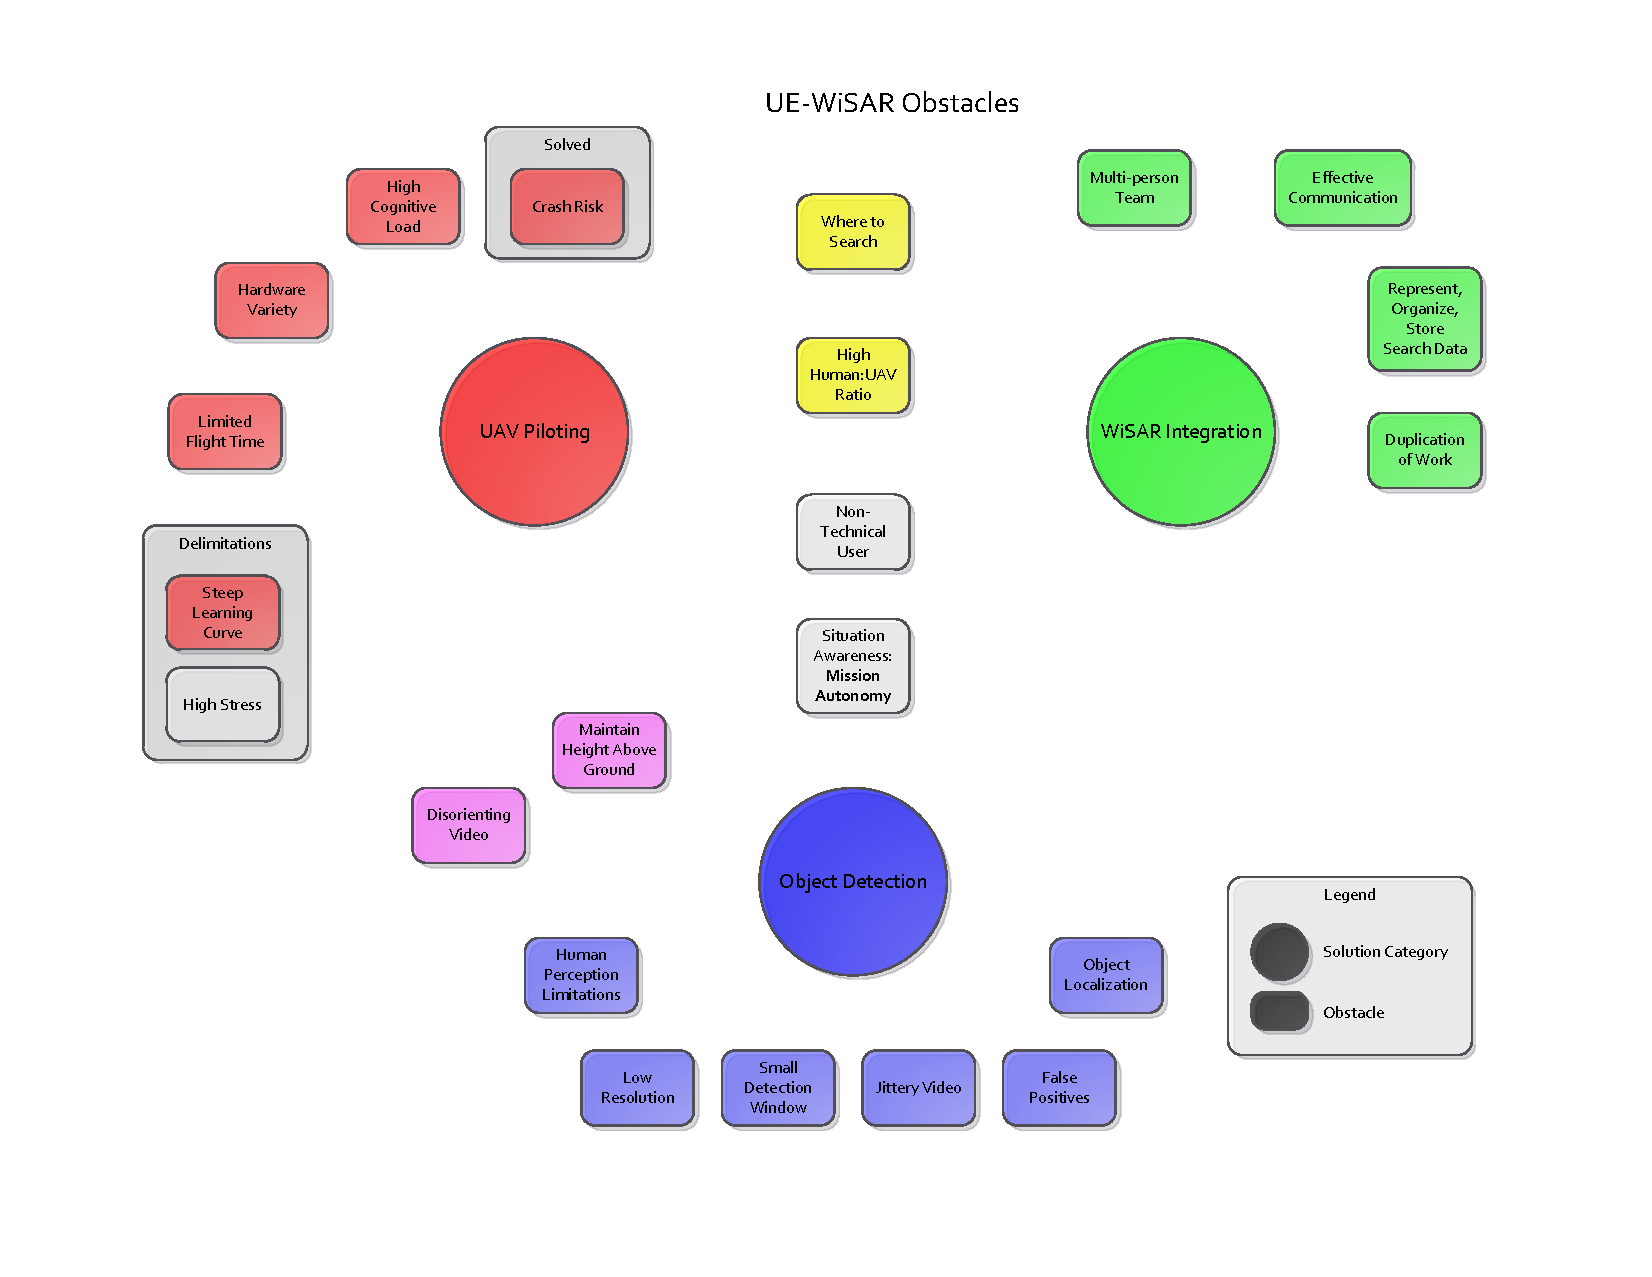
\includegraphics[keepaspectratio=true, width=\paperheight,
	height=\paperheight, page=1, angle=90, scale=0.95,
	trim=20 0 20 0]{obstacle_solution_map.pdf}
	\caption{UE-WiSAR Obstacles}
	\label{fig:obstaclemap}
\end{figure*}


\subsection{UAV Piloting}

\textbf{High Cognitive Load}.  mUAVs operate under multiple
degrees of freedom which can be disorienting for pilots.  A high level of
concentration is required to avoid becoming confused while piloting.  This is
somewhat mitigated by the low-level autonomy that this project builds upon
\cite{lin2010supporting}.  However, a fair amount of cognitive load is still
required.  Path-planning, status monitoring and team communication are tasks
that must still be addressed.

\textbf{Hardware Variety}.  The variety of hardware that can be used for mUAVs
is constantly increasing.  For any system to be viable as a perpetual framework
for UAV research it must have mechanisms in place to allow for the piloting of any number of unique mUAVs.

\textbf{Limited Flight Time}.  Most battery-powered mUAVs are limited to a
flight time of under 120 minutes, many are much less.  This limitation makes flight
planning much more difficult and introduces the potential for critical failure
during a flight.

\subsection{Object Detection}

\textbf{Human Perception Limitations}.  To be successful human
users must be able to detect objects on screen.  This implies that video presented to users
will only be effective if it accounts for the limitations of the human
eye \cite{humphrey2009human}. The eye is only able to discern high detail with
the cones located in the center.
This means that to detect an object the user must be looking almost directly at
the object while it moves across the screen.  Another limitation is that 
the eye has difficulty detecting small changes in intensity, an effect that gets
worse as brightness goes down \cite{gonzalezwoodsDIP}.

\textbf{Low Resolution}.  The video resolution is a result of
current hardware.  The mUAVs at this time broadcast NTSC 640x480 resolution. 
This resolution makes it extremely difficult to locate small objects which may be represented by only
a few pixels \cite{goodrich2009towards}.

\textbf{Small Detection Window}.  When using a fixed wing mUAV the video
captured is in constant motion.  This motion means that a potential target will
only remain visible for a short time.  Minimum mUAV flight speeds only slightly
improve the detection window and cannot fully correct this
problem \cite{goodrich2009towards}.

\textbf{Jittery Video}.  For stable flight, the mUAV is constantly correcting
course through small adjustments.  These adjustments occasionally have the
undesired effect of making video appear jittery.  This problem is magnified
in adverse weather conditions \cite{goodrich2009towards}.

\textbf{Object Localization}.  Assuming an object
has been detected in surveillance video the next step in a WiSAR operation is to send ground
searchers to the object.
In a May 2008 field trial, video analysts where unable to accurately communicate
the location of an object and had to observe the searchers from the mUAV to give
them directions relative to the object \cite{goodrich2009towards}.  This example
illustrates a different challenge which is determining the exact location of a
detected object.

\textbf{False Positive Detections}.  Due to the cost associated with missed
detection, a human life, a high false alarm rate is considered tolerable.  If
the false alarm rate is too high, however, it degrades the practicality of the
tactic.  On top of that each false alarm requires effort that may bog down the
search or leach resources from other tactics \cite{goodrich2008supporting}.

\subsection{WiSAR Integration}
The next group of obstacles fall under the WiSAR Integration category and
represent the challenges from introducing mUAVs into a WiSAR operation.
A cognitive task analysis was performed to provide
insights for such an integration  \cite{adams2009cognitive}.  The goal directed
task analysis and work domain analysis from this effort communicate how complex a
WiSAR operation is.  To integrate with such a complex endeavor a few obstacles
must be overcome.

\textbf{Multi-Person Team}.  WiSAR operations are made up
of potentially hundreds of people.  Additionally, the mUAV requires its own
team.  Not only must the mUAV team operate as a team but it must also interact
with the overall operation.  These multi-person, multi-team environments often
generate role confusion, conflict, and inefficiency
\cite{goodrich2008supporting}.

\textbf{Effective Communication}.  No search can be
effective without the relevant data.  A typical WiSAR operation uses a
hierarchical command structure.  The mUAV team must be able to fold into the
hierarchy such that it receives relevant search data.  The mUAV team must then
communicate internally as individual roles are performed.  Important information
must then be communicated back into the parent command structure.

\textbf{Representing, Organizing, and Saving Search Data}.  The data provided to
the mUAV team must be interpreted so that it can be understood by the mUAV.  Additionally the data
provided by the mUAV must then be interpreted so it can be understood by users
and commands further up the chain.  This implies an internal data organization
associated with the mUAV.  This organization must facilitate the storing and
sharing of said data.

\textbf{Duplication of Work}.  This mostly applies to search area coverage. 
The mUAV team must be able to track what it has searched and how well it
was searched.  Without this information search planning will be inaccurate which
could have fatal consequences.

\subsection{UAV Piloting \& WiSAR Integration}

\textbf{Where to Search}.  During a WiSAR
operation the probability of area (POA) \cite{koester2008lostpersons} is
constantly changing as new information is acquired.  For a UAV to integrate into
a WiSAR operation it must have the ability to interpret this information, act on
information, and contribute information.  If information is lacking then it must
be able to generate information to act upon.  A target can only be spotted by
the mUAV if it shows up on the video.

\textbf{High Human to UAV Ratios}.  This obstacle is based on practicality.  It
is not practical to require a large team for a single mUAV.
With the variety of tasks that emerge when introducing a mUAV to WiSAR it
becomes quite challenging to keep this ratio down.  A study by Cooper 
\cite{cooper2008towards, goodrich2009towards} speculates that it may be possible
for a single human to simultaneously navigate an area while localizing objects. 
His conclusion outlines several requirements he feels must be met before this
can become reality.  This becomes even more challenging when considering the
Mision Manager role as well.

\subsection{UAV Piloting \& Object Detection}
\textbf{Maintaining Height Above Ground (HAG)} \cite{adams2007camera}.
This represents one of the major crash risks associated with user error.  In an
early test flight the pilot placed two way points of similar HAG a fair distance
apart.  As the mUAV flew between the way points it crashed into a tall ridge
that separated the waypoints.  The pilot wasn't aware that his flight path went
through the ridge. This example illustrates one reason for maintaining HAG;
another reason is related to Object Detection.
Goodrich et al. state that the minimal resolution
of an image for detecting a human form is 5cm per pixel
\cite{goodrich2008supporting}.  This means that an image can cover an area no wider than
32m and 24m tall.  They go on to suggest that the
maximum HAG be between 60m to 100m.

\textbf{Disorienting Video}.  Disorienting video is produced when the mUAV is
performing manuevers which change the camera field of view and cause the user to feel
disoriented \cite{morse2008application}.  Even small manuevers can be
disorienting when occurring in succession.
This is a challenge because the UAV cannot obtain the needed surveillance
without turning.  Also, the light weight of the mUAV causes it to be
susceptible to wind which can cause excess manuevering.

\subsection{Universal Obstacles}
\textbf{Non-Technical Users}.  For UE-WiSAR to be
practical it must strive to be accessible to the greatest number of users.  With
this said UE-WiSAR is a technical operation and cannot be divorced completely
from its technical aspects.  UE-WiSAR requires some knowledge of mUAVs,
networking, and radio transmission. The real obstacle is segregating
and limiting the technical experience required for UE-WiSAR into as few roles as
possible.

\textbf{Situation Awareness}.  This represents the user's ability to maintain
awareness of the bigger picture while performing tasks.  This is broken into
two categories.  The first category relates to the mission.  The main goal of
any UE-WiSAR operation is to find the missing person.  If the tasks performed by
mUAV team members require a cognitive load that is too high team members will be
unable to meet their respective responsibilities which may have tragic
consequences to the search.  The second category relates to autonomy.  Autonomy
is a central concept to UE-WiSAR.  As autonomy increases certain negative
attributes can emerge  \cite{adams2007camera}, including:
\begin{itemize}
	\item Reduced situational awareness
	\item Difficulty in supervising autonomy
	\item Increased interaction time
	\item Increased demands on the human and autonomy
\end{itemize}
As autonomy decreases the following negative attributes
can emerge \cite{cooper2006integrating}:
\begin{itemize}
	\item High cognitive load on operator
	\item Steep learning curve
	\item Increase pilot:UAV ratio
\end{itemize}
The balancing of this dynamic relationship between the autonomous and
operator-controlled elements of UE-WiSAR is important because it is directly
linked to the usability of the solution.

\begin{figure*}[htp]
	\vspace{-80pt}
	\hspace{-90pt}
	\includegraphics[keepaspectratio=true, width=\paperheight,
	height=\paperheight, page=3, angle=90, scale=0.95,
	trim=10 0 10 0]{obstacle_solution_map.pdf}
	\caption{UAV Piloting Solutions}
	\label{fig:uavpilotingmap}
\end{figure*}

\section{SOLUTIONS}
The solutions to the above mentioned obstacles are organized into three categories.
See Figure~\ref{fig:obstaclemap} on page
\pageref{fig:obstaclemap}.  This organization is preferred because many of
the solutions discussed here solve problems associated with multiple obstacles. 

As mentioned earlier, these solutions already exist in different states.  The
subsequent paragraphs will expand on the work required to add the solution to
UE-WiSAR.

\subsection{UAV Piloting}
This solution category focuses on overcoming obstacles
associated with piloting the mUAV.  See Figure~\ref{fig:uavpilotingmap} on page
\pageref{fig:uavpilotingmap}.


% \begin{figure*}[htp]
% 	\label{fig:uavpilotingmap}
% 	\includegraphics[keepaspectratio=true,	height=1.0\textwidth, angle=90, page=3]{obstacle_solution_map.pdf}
% \end{figure*}

\textbf{Automated Flight Paths (AFP)}.  The first obstacle this addresses is the
high cognitive load on the pilot.  Detailed flight paths can be generated in a matter of
moments with minimal user input.  These flight paths can also be adjusted based
on the limited flight time.  Lin has created an algorithm
that when given a probability distribution map, start point, end point and
flight time will generate a flight path that maximizes the mUAV cameras coverage
of the probability distribution \cite{lin2009uav}.  Another type of flight path
is the Generalized Contour Search \cite{goodrich2008supporting}.  This flight
path requires a gimbaled camera but also generates optimal search patterns for certain
conditions.  Automatically generated flight paths can also attempt to limit the
number of turns made by the UAV to minimize the amount of disorienting video
captured during a flight.  Lastly, these flight paths can use HAG information to
maintain the optimal HAG for object detection while also avoiding obstacles such
as ridges or cliffs.

\textbf{Pre-Load Terrain Data}.  Terrain data provided by a number of sources
can be downloaded over the internet prior to the search.  This data is critical for
implementing effective AFPs and POA distributions.

\textbf{Modular Hardware Interface}.  To overcome the hardware variety obstacle
UE-WiSAR will use piloting interfaces that must be implemented for specific technologies.
While the initial UE-WiSAR release will have limited hardware support, namely
Procerus and Mikrocopter, more support can be added through implementing a
single interface for the specific technology.  This approach minimizes the work and knowledge required to adapt
the software to new hardware.

\textbf{UE-WiSAR Pilot UI}.  This user interface has two main
requirements \cite{lin2010supporting}.  First is assigning tasks to the mUAV. 
This implies an ability to make the mUAV an effective part of the search by
having the mUAV capture high quality video footage of regions specified by the
incident commander.  It does not imply deep understanding of mUAV piloting,
flight path automation, or other technical details associated with piloting a
mUAV \cite{cooper2007supporting}.

The second requirement is the ability to monitor the health of the mUAV.
This means the UI must communicate the exact position and status of the mUAV at
all times and alert the pilot when user input is required.  Because this UI
is the main focus point for the pilot, it is a primary concern for loss of
situation awareness.  To avoid this the UI must be able to dynamically adjust
the amount of automation needed as dictated by the situation.

\subsection{Object Detection}
This section focuses on detecting objects
in video captured by the mUAV.  See Figure~\ref{fig:objectdetectionmap} on page~\pageref{fig:objectdetectionmap}.

\begin{figure*}[htp]
	\vspace{-55pt}
	\hspace{-80pt}
	\includegraphics[keepaspectratio=true, width=\paperheight,
	height=\paperheight, page=4, angle=90, scale=0.90,
	trim=20 0 20 0]{obstacle_solution_map.pdf}
	\caption{UAV Piloting Solutions}
	\label{fig:objectdetectionmap}
\end{figure*}
% \begin{figure*}[htp]
% 	\label{fig:objectdetectionmap}
% 	\includegraphics[keepaspectratio=true,	height=1.0\textwidth, angle=90, page=4]{obstacle_solution_map.pdf}
% \end{figure*}

\textbf{Temporally Localized Mosaic} \cite{morse2008application,
cluff2009unified}.  This process allows the user to view the current frame in relation to a history of previous frames.  An object that appeared in a
single frame may now remain visible for multiple frames.  Morse et al. conducted
user studies to analyze the effectiveness of this
approach.  Those studies found a 43\% improvement in
hit probability when using mosaiced views versus non-mosaiced views.  While
there was an increase in false positive detections this increase is considered
inconsequential along side the improvement to hit probability.

\textbf{Spectral Anomaly Detection} \cite{thornton2011detection,
rasmussen2008enhancement}.  In typical WiSAR video the majority of colors are
varying shades of grey, brown, and green.  This process looks for objects that
are ``out-of-place''.  This autonomous detection will not replace user
detection, instead it aids user detection by suggesting objects to the user for
closer inspection.

\textbf{GPS Frame Referencing} \cite{morse2010coverage}.  This process uses
geometry to map pixels to gps coordinates.  The
algorithm uses the GPS coordinates of the mUAV, mUAV position, terrain data,
and camera specifications to determine the relation of the point to the UAV. 
While the process is simple, it suffers from the limited precision of mUAV
sensors and may provide highly inaccurate locations.

\textbf{Video Analyst UI} \cite{lin2010supporting}.  This UI is meant for users
operating under the Video Analyst Role.  Its purpose is to help Video
Analysts detect objects seen by the mUAV.  There are three main requirements
associated with accomplishing this purpose.  The first is to provide video to
the user.  As a search progresses Video Analysts may need to analyze live video,
video of specific areas, or video from certain times.  The UI must make it easy
for analysts to find the video that needs to be analyzed.  The second
requirement is to aid in object detection.  The UI must be able to enhance the
video as directed by the user.  This includes the above mentioned solutions
along with other simple enhancements such as brightness, contrast, and rate of
playback.  The last requirement is that the UI allow the analyst to communicate
with the mUAV team.  As an analyst works they must be able to communicate
findings to the mUAV team.

\subsection{WiSAR Integration}
WiSAR Integration focuses on introducing a mUAV to a
WiSAR operation.  See Figure~\ref{fig:wisarintegrationmap} on
page~\pageref{fig:wisarintegrationmap}.

\begin{figure*}[htp]
	\vspace{-90pt}
	\hspace{-80pt}
	\includegraphics[keepaspectratio=true, width=\paperheight,
	height=\paperheight, page=2, angle=90, scale=0.95,
	trim=10 0 10 0]{obstacle_solution_map.pdf}
	\caption{WiSAR Integration}
	\label{fig:wisarintegrationmap}
\end{figure*}
% \begin{figure*}[htp]
% 	\label{fig:wisarintegrationmap}
% 	\includegraphics[keepaspectratio=true,	height=1.0\textwidth, angle=90, page=2]{obstacle_solution_map.pdf}
% \end{figure*}

\textbf{Team Roles} \cite{goodrich2008supporting,adams2009cognitive,goodrich2007using}.  UE-WiSAR will use a hierarchical command structure.
The top level role is the \emph{Mission Manager} (MM).  The MM is responsible
for defining the search in UE-WiSAR.  The MM is also responsible for directing
the other roles associated with a mUAV search.

The next role is \emph{UAV Pilot}.  The Pilot is responsible for capturing video with the
mUAV as directed by the MM and communicating important information about the
status of the mUAV to the MM.  

The last role is \emph{Video Analyst}.  The
Analyst is responsible for detecting objects in the captured video.
The Analyst communicates any findings to the MM.  

This role breakdown enables a
mUAV team of two or more people to operate effectively through a clean breakdown
of work and established communication channels.

\textbf{Independent Technical Search Team}
\cite{adams2009cognitive}.
UE-WiSAR represents a single search tactic for locating missing persons.  This
implies that UE-WiSAR will be used as part of a larger WiSAR operation.  This is
facilitated through the MM role.
The MM is responsible for obtaining the missing person data and entering the
data into UE-WiSAR.  The MM is then responsible for constructing a mUAV search
plan as directed from the chain of command.  As the mUAV team follows the
search plan, everything is reported back to the MM who then relays relevant
information back to the main chain of command.

\textbf{Command \& Control UI} This UI is meant for users operating under the
Mission Manager Role.  Its purpose is to facilitate the MM responsibilities. 
There are three main requirements for accomplishing this purpose.  The first is the ability to build a missing person profile. 
Information such as the last known location, clothing color, destination,
starting point, etc. is essential for the automation and the mUAV team. 
The UI must allow the MM to enter this data but not overload the MM with tedious
data entry.  The next requirement is the ability to define a search plan.  The
UI must show relevant search data to the MM and allow the MM to define a search
plan which can then be carried out by the Pilot.  The
last requirement is the ability to receive communications from mUAV team members.  The UI must alert the
IC of detected objects, mUAV status, search progress.  The UI must also
communicate this information in a way that it can be presented to the main chain
of command.  Additionally the UI must be intuitive, clean, and simple.

\textbf{Distributed System Design}  A client-server architecture has been chosen
for UE-WiSAR for several reasons.  The first reason is the computational load
required to enhance video received by the mUAV.  The resources needed are much
greater than those of a typical desktop computer and require a powerful server. 
Once the video has been enhanced, however, it can be distributed to clients at
little cost.  Another reason for this architecture is the unknown team size. 
Collected video must be analyzed by the human-eye.  This architecture allows for
any number of video analysts to work symultaneously, assuming there is enough bandwidth.
Another reason for this architecture is to simplify the software.  Instead of
building an all-in-one software solution, a server and multiple independent
client applications can be written.  Clients can then choose which application
to run according to their roles which in turn makes the client roles less
confusing.

\textbf{Video Annotations}  These are the primary means of communication for the
Analysts.  When an Analyst detects an object they can click on the object and
create an annotation.  The annotation will then carry information about that
object such as location, time of discovery, place in video, analyst comments,
priority, etc.  Once an annotation is created it instantly becomes
available to other team members, in the case of the IC, alerting them of the
annotation.  The annotation can then be modified as needed depending if it was a
false alarm or a real sign.  If an annotation is a real sign it can be converted
to a format acceptable to the external chain of command.

\textbf{Persistent Incident Management}  Essentially this refers to a relational
data model specifically designed for UE-WiSAR.  The root node of this data model
will be an incident, all other data will be linked to an incident.  The model
will hold missing person data, search plans, flight plans, videos, annotations,
etc.  Storing data in the model will reduce work duplication and make
data more accessible.  The model will also simplify persistent storage as xml
files or a sql database.  In concert with the project goals this data model can
be shared with other search groups and search databases to help improve WiSAR.

\textbf{See-Ability} \cite{engh2008see}  This is a method of determining how
well an area has been searched by the mUAV.  The algorithm uses the position of the
camera in relation to the ground to determine the quality of the view.  This can
later be used to find how many times a location has been viewed, how many unique
angles has it been viewed from, and what is the overall quality of the viewings.
This can be a great help to the MM and Pilot in avoiding over-viewed areas,
narrowing search parameters, and maintaining situation awareness.

\textbf{POA Models} \cite{koester2008lostpersons}  Because UE-WiSAR must
be able to act independently, two probability of area models will be added
to the CC interface.  The first is the Segment Model.  This model allows the IC
to strategically breakdown a large search region into smaller search regions. 
Efforts can then be focused on high priority regions as directed by the IC.  The
second model is the Ring/Dispersion Model.  This model uses the last known
location along with the intended destination to create an ever expanding search
corridor with eminating rings that occur at specific distances.  The
highest POA occurs inside the corridor and inside the first ring, then second
ring, etc.


\section{DELIVERABLES}
As an industrial thesis a major goal is to produce high quality software that is
on par with industry standards.  Quality as it relates to the project goals is
the users ability to perform tasks within their roles and to allow future
developers to understand UE-WiSAR well enough to modify/enhance the software as
needed.  To following descriptions of work will be used to validate that the
project goals have been met and that the project is a success.

Therefore, the first deliverable will be a detailed list of requirements
organized into groups and prioritized.  Glass's law states that ``Requirement deficiencies are the prime source of project failures.''  The list of requirements is meant to be an ideal goal.
Not every requirment will be acheived, and some may change, instead it is meant
to be a road map.  By clarifying the project requirements early the student and
committee members can make informed decisions, avoid mistakes, and measure progress.
It is also expected that design specifications will improve the design and make
prototyping more effective.  

The second deliverable will be detailed design documents specifying the
architecture, data model, workflows, dataflows, protocols, user manuals and
language/framework considerations.  These documents will make up a collection
of text, UML, and other documents.  Their purpose is to clarify how the system
works and how it accomplishes project goals.  Boehm's first law states ``Errors are most frequent during the requirements and design activities and are the
more expensive the later they are removed."  This step of the project will help
to reduce bugs and development time by allowing for peer review and prototyping
before major work is done.  Many of these documents are living documents and
will change as the project progresses, some may not exist until after coding
has been completed.  It is expected that requirements and design will take up to
one third of the total project time.

The third deliverable will be the actual UAV Enabled Wilderness Search and
Rescue code.  The code will be well documented, follow consistent coding
practices, and compile on designated operating systems.  This represents the
majority of work done on the project.

The fourth deliverable will be a demonstration of the software in a
live environment with a real mUAV and controlled targets.  This demostration
will show that core features exist, the software is stable, and users are able to perform tasks by following written
instructions.  Core features are the set of features decided on by the student
and committee that the software must have to be considered functional.  The
users will be individuals, preferably familiar with WiSAR, unfamiliar with
operating the UE-WiSAR software.  At least one user per role will be involved. 
An experienced mUAV pilot will also be involved to reduce risk to equipment. 
Basic tasks will be assigned that require use of the core features.  This will
not be an exercise in validating prior research.

% \section{Specification of Work}
% As mentioned, a substantial amount of work has already been done in
% consolidating the prototype code and implementing the proposed project.  The
% current WonderServer project, developed in C++ on the QT framework, has a
% Server, Pilot UI, and Video Analyst UI \cite{uavCode, serverCode}.  While each
% component is incomplete, stable network communication, open GL integration, and mUAV Hardware communication are working.  The ability
% to perform these basic tasks proves the capability of the chosen framework.  The
% next step is to engineer the software to maximize the potential to fulfill its
% goals.  The Model View Controller (MVC) design pattern will represent the
% overall design.  This is ideal because UE-WiSAR has a minimum of four UIs that will all
% interact with the same Model.  To fit UE-WiSAR to the MVC pattern the following
% tasks must be completed.
% 
% \textbf{Data Model}  A Data Model will be designed to store information for a
% WiSAR incident.  All data that is relevent to the system will be represented in
% the Data Model.  The model will be responsible for assigning unique id's to
% objects and maintaining data integrity of the objects it stores.  To simplify
% model interaction the Facade pattern will be used both in and around the model
% wherever the logic becomes moderately complex.  The model will use appropriate
% design patterns to represent the data.
% 
% \textbf{Data Persistence}  Beneath the Model layer a Data Persistence layer will
% exist that can convert the Model into a persistent medium.  Initially this will
% be as serialized data files, however, the design allows for the addition of
% other mediums such as SQL without impacting the system.
% 
% \textbf{Controllers}  The controllers are responsible for communicating between
% the Model and the View.   Because the View can be on a different machine than
% the Model this communication is more complex.  Views will be expected to
% maintain their own custom models.  The controller will be responsible for
% syncing the data in these models as necessary.  A client controller will
% interact with a sibling controller on the server as needed through a network
% interface.  Interfaces must be created for all Controllers before the
% controllers are created.
% 
% \textbf{Views}  Interfaces must be created for all Views before the Views are
% created.  Each UI is made up of one or more Views and can become confusing. 
% Interfaces are pre-designed so that when implemented will ensure all required
% features are met.  A general idea of the requirements for each view are as
% follows:
% 
% \begin{itemize}
% 	\item \textbf{Server}
% 	\begin{itemize}
% 	  \item Add/Edit mUAV Hardware Connections
% 	  \item Add/Edit an Incident
% 	  \item View Terrain Data
% 	  \item View Video
% 	\end{itemize}
% 	
% 	\item \textbf{Command \& Control UI}
% 	\begin{itemize}
% 	  \item Add/Edit an Incident
% 	  \item Add/Edit POA Models
% 	  \item View Terrain Data
% 	  \item View See-Ability
% 	  \item View Annotations
% 	  \item View Video
% 	\end{itemize}
% 	
% 	\item \textbf{Pilot UI}
% 	\begin{itemize}
% 	  \item Add/Edit mUAV Hardware Connections
% 	  \item Add/Edit Flight Paths
% 	  \item View Terrain Data
% 	  \item View Search Areas
% 	  \item View Annotations
% 	  \item View mUAV Status
% 	  \item View Live Video
% 	\end{itemize}
% 	
% 	\item \textbf{Video Analyst UI}
% 	\begin{itemize}
% 	  \item View Video
% 	  \item Add/Edit Annotations
% 	  \item View Incident Information
% 	\end{itemize}
% \end{itemize}
% 
% There is also work that must be done outside of the MVC structure.  Most of the
% autonomous solutions that will be implemented integrate with the Data Model,
% however, they exist separate from the MVC design.
% These solutions will be implemented as independent libraries that will be used
% by the Data Model and Controllers as needed.  An example of this is Automatic
% Flight Path Generation, Mosaicing, Anomoly Detection, etc.  The status of
% these libraries was described previously.

% \subsection{Time to Complete}
% An important concern is the time to complete this project.  It is possible that
% not everything can be coded in the time alloted.  With this consideration it is
% important to recognize what aspects of the software are required to consider the
% project a success.  
% 
% The first of the requirements is the porting of prototype code into individual
% QT libraries.  These libraries represent the intelligence and automation behind
% the UE-WiSAR software and are a major part of the research done here at BYU. 
% This includes but is not limited to Mosaicing, See-Ability, Anomoly Detection,
% Flight Path Generation, POA Modeling, and UAV communication.
% 
% The second requirement is the UE-WiSAR Server.  The server is responsible
% for collecting and storing data from mUAVs, Video Streams, External Map
% Sources, GUI's, and UE-WiSAR clients.  As data comes in from these sources the
% server uses the above mentioned libraries to extrapolate more data.  This is the
% backbone of the UE-WiSAR project and must be completed.  For detailed
% requirements look at 
% 
% The last requirement to mark the project successful is for user validation of
% the features described in this proposal.  This represents the CC, Pilot, and
% Video Analyst Clients.  These clients must be developed enough that a user
% familiar to WiSAR can perform a search and verify that the described features
% exist and work.  The user interfaces will be what suffer the most if time
% becomes short.  The reason this is acceptable is because the clients implement the Controller and View interfaces
% which make them easily replaceable.  New GUI's can be created as needed that
% implement the same interfaces but which look and feel much more polished with
% little to no consideration to backend operation.  In fact it is expected that
% when released most community contributions will be in the form of GUI
% enhancements.

% \section{Validation}
% There are two aspects to the validation of the project.  The first is validation
% of the quality of the software.  As an industrial thesis a major goal is to
% produce software that is on par with industry standards.  This will be
% accomplished through documentation.  Comments will be included on each class
% that describe the purpose of the class and what it does.  Using Doxygen this
% data will be compiled into detailed class documents.  Also, design documents
% describing the Data Model, Design Patterns, WiSAR Integration and Usage of key
% features will be created.
% 
% The second validation aspect will be the verification of the minimum set of
% requirements.  Monthly design review meetings will be held, if needed the
% requirements can be modified in these meetings.  The minimum list of
% requirements will be verified by an individual familiar with the UE-WiSAR
% software.  If the user can perform the minimum requirement list then the
% software will be considered validated.  See Figure~\ref{fig:serverrequirements}
% on page~\pageref{fig:serverrequirements}.
% 
% \begin{figure*}[htp]
% 	\caption{Detailed Server Requirements}
% 	\begin{itemize}
% 		\item \textbf{Incident Information}
% 		\begin{itemize}
% 		  	\item Manage Search Incidents
% 		  	\begin{itemize}
% 			  	  \item Incident Area
% 			  	  \item Missing Person Profile
% 			  	  \item Last Known Locations
% 	  	  	\end{itemize}
% 	  	  	\item Load existing Search Incidents
% 	  	  	\item Switch between Incidents
% 	  	  	\item Generate POA models from Missing Person Data
% 	  	  	\item Automatically Download Terrain Data for Incident Area
% 		\end{itemize}
% 		
% 		\item \textbf{Terrain Data}
% 		\begin{itemize}
% 			\item Obtain Third Party Map Data for a specified incident area.
% 	  		\begin{itemize}
% 	  		  	\item MapQuest Image Tiles
% 	  		  	\item OpenMaps Image Tiles
% 	  		  	\item USGS NED 1/3 GridFloat
% 	  		  	\item USGS LandCover GridFloat
% 		  	\end{itemize}
% 		  	\item Save Terrain Data to disk
% 		  	\item Make Terrain Data available to clients
% 		  	\item Perform fast queries on Terrain Data
% 	  		\begin{itemize}
% 	  		  	\item HAG of specific coordinate
% 	  		  	\item LandCover of specific coordinate
% 		  	\end{itemize}
% 	  		\item Manage Incident Map Objects
% 			\begin{itemize}
% 			  \item Points
% 			  \item Areas
% 			  \item Custom Objects
% 			\end{itemize}
% 		\end{itemize}
% 		
% 		\item \textbf{Video}
% 		\begin{itemize}
% 	  		\item Manage Camera Profiles
% 	  		\item Capture Video Frames
% 	  		\begin{itemize}
% 	  	 		\item Save Frames to Harddrive
% 	  	  		\item Save GPS Location of Frame
% 	  	  		\item Connect Frame to Incident
% 	  	  		\item Homography Calculation on Frame
% 	  	  		\item Anomoly Analysis on Frame
% 	  		\end{itemize}
% 		  	\item Stream Captured Video
% 		  	\item Manage Annotations
% 		\end{itemize}
% 		
% 		\item \textbf{UAV}
% 		\begin{itemize}
% 		  	\item Manage UAV Profiles
% 		  	\item Manage UAV Plugins
% 		  	\item Communicate with UAV
% 		  	\begin{itemize}
% 		  	  	\item Save UAV data to Harddisk
% 		  	  	\item Issue Commands to UAV
% 		  	  	\item Track UAV position
% 	  	  	\end{itemize}
% 	  	  	\item Generate Flight Paths
% 	  	  	\item Monitor UAV Status
% 	  	  	\item Manage See-Ability
% 		\end{itemize}
% 	\end{itemize}
% 	
% 	\label{fig:serverrequirements}
% \end{figure*}
\section{DELIMITATIONS}
Due to the nature of software development and the size of this project there
will be a large list of things to do that can be done in a reasonable amount of
time.  The goal of this project is not to implement the maximum amount of
features, instead the goal is to create a stable foundation for others to
implement the features they choose.  This is particularly relevent in regards to
user interfaces.  

This project will not create the ideal user interfaces as described in the
solution section as those are subjective and become much too time consuming. 
Instead the project will focus on functionality and creating basic user interfaces that can be
easily replaced by future developers.

The project also doesn't account for the High Stress that is associated with SAR
operations.  It is known that High Stress has a negative impact on an
individuals cognitive load capacity, however, it is too complicated to include in this proposal.  

There are several learning curves that are associated
with different aspects of this project.  Because learning curves are unavoidable
and vary with the individual it is enough for this proposal that the software is
targeted at as large a user group as possible.

There are too many unknowns to accurately predict the amount of time a project
this size will take to complete.  The focus will be on the deliverables and
working closely with advisors during the development process to adjust the
requirements to fit with time constraints.

\section{CONCLUSION}
UE-WiSAR represents an opportunity for the research done at BYU to serve a
greater community.  As Thomas Edison once said ``The value of an idea lies in
the using of it.''  UE-WiSAR will not only provide a new search Tactic for
SAR operations, it also provides a framework for mUAV enthusiasts and
researchers to build upon for continued research in the field.  What now exists
as a collection of interesting ideas will become the do-it-yourself manual for
performing aerial surveillance using mUAVs.  

Unlike many open source solutions, the focus of creating software at current
industry standards makes UE-WiSAR even more valuable.  With good design and
documentation the project is much more likely to take hold in the open source
community further increasing its ability to serve those communities it is meant
to serve.